% Synchronized to r34917

\marklabel{chap:bootmedien}{
  \chapter{Creating the fli4l Archives/Boot media}
  }

  If all configuration is completed, the fli4l archives/boot media may be created
  as either bootable Compact-Flash, a bootable ISO image, or only the files needed
  for a remote update.

\marklabel{sec:bootmedien_linux}{
  \section{Creating the fli4l Archives/Boot media under Linux or other Unix derivatives and Mac OS X}
  }

  This is done by using scripts (\texttt{.sh}), which can be found in the
  fli4l root directory.

  \begin{description}
    \item \texttt{mkfli4l.sh}
  \end{description}

  The Build Script recognizes the different \jump{BOOTTYPE}{boot types}.

  The simplest call on Linux looks like this:
   \begin{verbatim}
    sh mkfli4l.sh
  \end{verbatim}

  The actions of the build scripts are controlled by three mechanisms:
   \begin{itemize}
    \item Configuration variable \var{BOOT\_TYPE} from
          \texttt{$<$config$>$/base.txt}
    \item Configuration file \texttt{$<$config$>$/mkfli4l.txt}
    \item Build-Script Parameters
  \end{itemize}

  The variable \jump{BOOTTYPE}{\var{BOOT\_TYPE}}
  decides which action of the Build Scripts is executed:
  \begin{itemize}
    \item Create a bootable fli4l CD-ISO-Image
    \item Generating the fli4l files needed for a remote update
    \item Generating the fli4l files and directly do a remote update via SCP
    \item a.s.o.
  \end{itemize}

  The description of the variables in the configuration file
  \texttt{$<$config$>$/mkfli4l.txt} can be found in Chapter
  \jump{sec:mkfli4lconf}{Control file mkfli4l.txt}.

  \subsection{Command line options}
  The last control mechanism is appending option parameters
  to the call of the Build Script on the command line.
  The control options correspond to those in the file \texttt{mkfli4l.txt}.
  Option parameters override the values from the control file.
  Out of convenience, the names of the option parameters differ from the names of
  the variables from the control file. There is a long and, to some extent, a
  short form:

  \begin{verbatim}
Usage: mkfli4l.sh [options] [config-dir]

-c, --clean         cleanup the build-directory
-b, --build <dir>   set build-directory to <dir> for the fli4l-files
-h, --help          display this usage
--batch             don't ask for user input

config-dir          set other config-directory - default is "config"

--hdinstallpath <dir> install a pre-install environment directly to
                    usb/compact flash device mounted or mountable to
                    directory <dir> in order to start the real installation
                    process directly from that device
                    device either has to be mounted and to be writable
                    for the user or it has to be mountable by the user
                    Do not use this for regular updates!

*** Remote-Update options
--remoteupdate        remote-update via scp, implies "--filesonly"
--remoteremount       make /boot writable before copying files and
                      read only afterwards
--remoteuser <name>   user name for remote-update - default is "fli4l"
--remotehost <host>   hostname or IP of remote machine - default
                      is HOSTNAME set in [config-dir]/base.txt
--remotepath <path>   pathname on remote maschine - default is "/boot"
--remoteport <portnr> portnumber of the sshd on remote maschine

*** Netboot options (only on Unix/Linux)
--tftpbootpath <path>   pathname to tftpboot directory
--tftpbootimage <name>  name of the generated bootimage file
--pxesubdir <path>      subdirectory for pxe files relative to tftpbootpath

*** Developer options
-u, --update-ver    set version to <fli4l_version>-rev<svn revision>
-v, --verbose       verbose - some debug-output
-k, --kernel-pkg    create a package containing all available kernel
                    modules and terminate afterwards.
                    set COMPLETE_KERNEL='yes' in config-directory/_kernel.txt
                    and run mkfli4l.sh again without -k to finish
    --filesonly     create only fli4l-files - do not create a boot-media
    --no-squeeze    don't compress shell scripts
    --rebuild       rebuild mkfli4l and related tools; needs make, gcc

    \end{verbatim}

   An HD pre-installation of a suitably formatted (FAT16/FAT32) CompactFlash
   (in a USB cardreader) or an USB Stick can be done by using the option
   \verb+--hdinstallpath <dir>+.
   You are using this script \emph{at your own risk}.
   The necessary fli4l files will be copied onto the specified partition.
   At first, run in the fli4l directory:

  \begin{verbatim}
     sh mkfli4l.sh --hdinstallpath <dir>
  \end{verbatim}
  \vspace{-2ex}
  This will generate the fli4l files and copy them to the CF-Card or USB Stick.

  To run the next steps, you have to make sure:

   \begin{itemize}
        \item \verb+chmod 777 /dev/brain+
        \item superuser rights
        \item installed \verb+syslinux+
        \item installed \verb+fdisk+
   \end{itemize}

 The script will ensure that this storage device is a FAT-partitioned USB-Drive.
 After that the boot loader and the files needed will be copied to the disk.
 You will get notified about success or failure.

 After the build you have to execute the following:

  \begin{verbatim}
    syslinux --mbr /dev/brain

    # make partition bootable using fdisk
    #     p - print partitions
    #     a - toggle bootable flag, specify number of fli4l partition
    #         usually '1'
    #     w - write changes and quit
    fdisk /dev/brain

    # install boot loader
    syslinux -i /dev/brain
 \end{verbatim}
 \vspace{-2ex}

 Now the CF resp. USB-drive should be bootable.
 Don't forget to unmount the device (via \texttt{umount}).

  \bigskip

  An alternative configuration directory can be specified by appending its name
  to the end of the command line. The normal configuration directory is called
  \texttt{config} and cn be found under the fli4l root directory. This is where all
  fli4l packages place their configuration files.
  If you want to maintain more than one configuration, create another directory, i.e. \texttt{hd.conf},
  place a copy of the configuration files there and change them according to the requirements.
  Here are some examples:

  \begin{verbatim}
     sh mkfli4l.sh --filesonly hd.conf
     sh mkfli4l.sh --no-squeeze config.test
  \end{verbatim}



\marklabel{sec:bootmedien_windows}{
  \section{Creating the fli4l Archives/Boot media under Windows}
  }

  Utilize the tool `AutoIt3' (\altlink{http://www.autoitscript.com/site/autoit/}). This enables a
  `graphical' edition, as well as dialogues which allow to change the variables described in the following
   sections.


  \begin{description}
    \item \texttt{mkfli4l.bat}
  \end{description}


  The Build program automatically recognizes the different \jump{BOOTTYPE}{boot types}.

  The `mkfli4l.bat' can be invoked directly from Windows Explorer, if you need no
  optional parameters.

   The actions of the Build program are controlled by different mechanisms:
  \begin{itemize}
    \item Configuration variable \var{BOOT\_TYPE} from the
          \texttt{$<$config$>$/base.txt}
    \item Configuration file \texttt{$<$config$>$/mkfli4l.txt}
    \item Parameter of the build program
    \item Interactive settings in the GUI
  \end{itemize}

  The variable \jump{BOOTTYPE}{\var{BOOT\_TYPE}} decides which action
  the Build program executes:
  \begin{itemize}
    \item Create a bootable fli4l CD-ISO-Image
    \item Making the fli4l files available, for remote update
    \item Generating the fli4l files and direct remote update via SCP
    \item Hard drive pre-install of a suitably formatted CF in the Cardreader
    \item a.s.o.
  \end{itemize}

  The description of the variables in the configuration file
  \texttt{$<$config$>$/mkfli4l.txt} can be found in Chapter
  \jump{sec:mkfli4lconf}{Control file mkfli4l.txt}.

  \subsection{Command line options}
  The last control mechanism is appending of option parameters to the call of the Build program
  on the command line. The control options correspond to those in the control file \texttt{mkfli4l.txt}. 
  Option parameters override the values from the control file.
  Out of convenience, the names of the option parameters differ from the names of
  the variables from the control file. There is a long and, to some extent, a
  short form:

  \begin{verbatim}
Usage: mkfli4l.bat [options] [config-dir]

-c, --clean             cleanup the build-directory
-b, --build <dir>       sets build-directory to <dir> for the fli4l-files
-v, --verbose           verbose - some debug-output
    --filesonly         creates only fli4l-files - does not create a disk
    --no-squeeze        don't compress shell scripts
-h, --help              display this usage

config-dir              sets other config-directory - default is "config"

*** Remote-Update options
--remoteupdate          remote-update via scp, implies "--filesonly"
--remoteuser <name>     user name for remote-update - default is "fli4l"
--remotehost <host>     hostname or IP of remote machine - default
                        is HOSTNAME set in [config-dir]/base.txt
--remotepath <path>     pathname on remote machine - default is "/boot"
--remoteport <portnr>   portnumber of the sshd on remote machine

*** GUI-Options
--nogui                 disable the config-GUI
--lang                  change language
                        [deutsch|english|espanol|french|magyar|nederlands]

  \end{verbatim}

  An alternative configuration directory can be passed by appending its name to the end of the command line.
  The normal configuration directory is called \texttt{config} and can be found under the fli4l
  root directory. This is where all fli4l packages place their configuration files.
  If you want to maintain more than one configuration, create another directory, e.g. \texttt{hd.conf},
  place a copy of the configuration files there and change it according to the requirements.
  Here are some examples:

  \begin{verbatim}
     mkfli4l.bat hd.conf
     mkfli4l.bat -v
     mkfli4l.bat --no-gui config.hd
  \end{verbatim}

  \subsection{Configuration dialog~-- Setting the configuration directory}

  In the main window the configuration directory setting is indicated and a window can be opened for
  the selection of the configuration directory.\\

  It should be noted that any change in the 'Config-Dir' causes all options to be set to the values contained in the
  \jump{sec: mkfli4lconf}{control file 'mkfli4l.txt'} placed in that directory, or to the values
  given as command-line parameters, respectively.\\

  If mkfli4l.bat does not find a directory fli4l-x.y.z$\backslash$config or if there is no file in that directory
  named `base.txt', a window is immediately opened for the selection of the configuration directory.
  This makes it possible to easily manage several fli4l configuration directories in a simple manner.\\

  Example:

\begin{example}
\begin{verbatim}
          fli4l-x.y.z\config
          fli4l-x.y.z\config.fd
          fli4l-x.y.z\config.cd
          fli4l-x.y.z\config.hd
          fli4l-x.y.z\config.hd-create
\end{verbatim}
\end{example}

  \subsection{Configuration dialog~-- General Preferences}
  \begin{figure}[ht!]
  \centering
  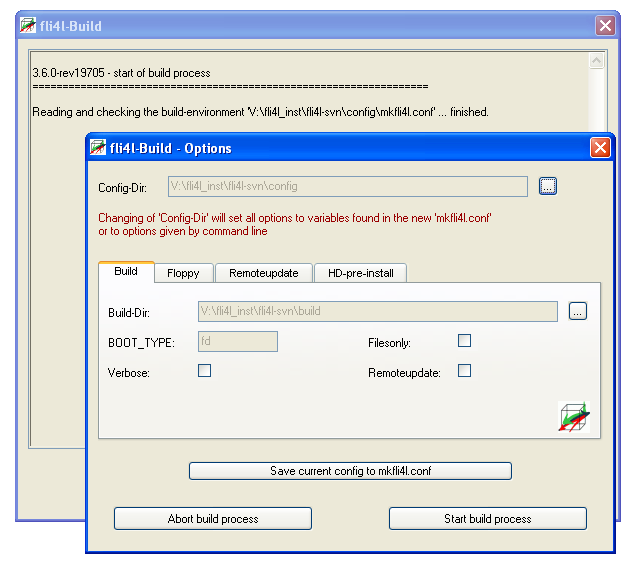
\includegraphics[width=\columnwidth]{win_build_build}
  \caption{Preferences}
  \label{fig:win_build_build}
  \end{figure}

  In this dialogue the settings are specified for the archive/boot-media
  creation:
  \begin{itemize}
    \item Build-Dir~-- Directory for the Archives/CD-Images/...
    \item \var{BOOT\_TYPE}~-- Display of the utilized/settings \var{BOOT\_TYPE}~-- unchangeable
    \item Verbose~-- Activation of additional output during the creation
    \item Filesonly~-- Only the archives are created~-- no bootmedia/no image
    \item Remoteupdate~-- Activation of the remote update via SCP
  \end{itemize}

  Using the button \textbf{Current settings in mkfli4l.txt buffer}
  the current settings can be stored in mkfli4l.txt.

  \subsection{Configuration dialog~-- Settings for Remote update}
  \begin{figure}[ht!]
  \centering
  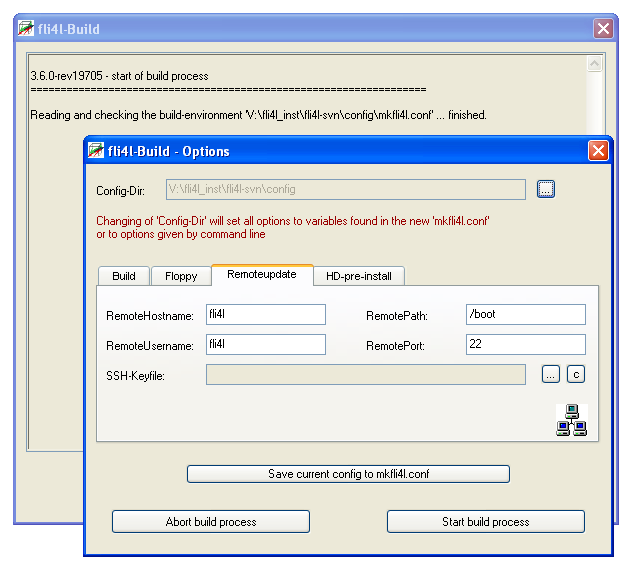
\includegraphics[width=\columnwidth]{win_build_remoteupdate}
  \caption{Settings for Remote update}
  \label{fig:win_build_remoteupdate}
  \end{figure}

  In this dialogue the settings for Remote update are specified:
  \begin{itemize}
    \item IP address or Hostname
    \item User name on the Remote host
    \item Remote path (default: /boot)
    \item Remote port (default: 22)
    \item SSH keyfile to use (format ppk from Putty)
  \end{itemize}

  \subsection{Configuration dialog~-- Settings for HD pre-install}
  \begin{figure}[ht!]
  \centering
  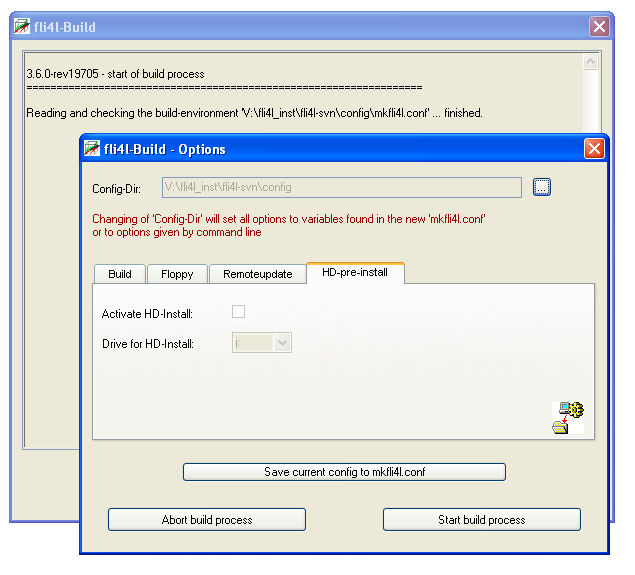
\includegraphics[width=\columnwidth]{win_build_hd_install}
  \caption{Settings for HD pre-install}
  \label{fig:win_build_hd_install}
  \end{figure}

   In this dialogue the options are set for HD pre-install on an
   accordingly partitioned and formatted Compact Flash card in a USB reader.

   Possible Options:
   \begin{itemize}
     \item Activate HD pre-install
     \item Drive letter to be used to access the CF card
  \end{itemize}

  Regarding the partitioning and formatting of the CF:
  A Type-A HD installation (see package HD) must be based on a primary, active,
  and formatted FAT partition on the CF card. If you would like to use a data partition
  additionally, a Linux partition which is formatted with the ext3 file system, as well as
  the file \texttt{hd.cfg} are also needed on the FAT Partiton (in this case please
  make sure to read the documentation of the HD package).

\marklabel{sec:mkfli4lconf}{
  \section{Control file mkfli4l.txt}}
  Since fli4l-Version 2.1.9 the control file
  \texttt{$<$config$>$/mkfli4l.txt} exists. This file can e.g. be used to specify
  directories which differ from the standard settings.
  The control file has a similar structure as the normal fli4l configuration files.
  All configuration variables here are optional, i.e. they need not exist or they can be commented out.
  \begin{description}

  \config {BUILDDIR}{BUILDDIR}{BUILDDIR}

  Default: `build'

  Specifies the directory where fli4l files will be created. If the variable is undefined,
  the Windows mkfli4l sets it to `build' relative to the fli4l root directory, resulting in
  the directory.
  \texttt{build} in the fli4l root directory:
  \begin{verbatim}
    Path/fli4l-x.y.z/build
  \end{verbatim}
  \vspace{-2ex}
  Under *nix mkfli4l is using \texttt{$<$config$>$/build} and is thus filing the
  generated files together with the configuration.

  The path for \var{BUILDDIR} must use the conventions of the Operating Systems
  Windows oder *nix. If relative paths configured there are converted by the build
  to the syntax of windows or *nix.

  \config {VERBOSE}{VERBOSE}{VERBOSE}

  Default: \var{VERBOSE='no'}

  Possible values are \var{'yes'} or \var{'no'}. Controls the \emph{Verbosity}
  of the Build Processes.

  \config {FILESONLY}{FILESONLY}{FILESONLY}

  Default: \var{FILESONLY='no'}

  Possible values are \var{'yes'} or \var{'no'}. This will actually
  turn off the creation of the boot-media and only the files will be created~--

  \config {REMOTEUPDATE}{REMOTEUPDATE}{REMOTEUPDATE}

  Default: \var{REMOTEUPDATE='no'}

  Possible values are \var{'yes'} or \var{'no'}. Enables automatic
  transferring of files by means of SCP to the router. This requires
  the package \jump{OPTSSHD}{SSHD} with activated \texttt{scp}.
  See also the following variables.

  \config {REMOTEHOSTNAME}{REMOTEHOSTNAME}{REMOTEHOSTNAME}

  Default: \var{REMOTEHOSTNAME=''}

  The target host name for the SCP data transfer.
  If no name is set, the variable
  \jump{HOSTNAME}{\var{HOSTNAME}} is used.

  \config {REMOTEUSERNAME}{REMOTEUSERNAME}{REMOTEUSERNAME}

  Default: \var{REMOTEUSERNAME='fli4l'}

  User name for the SCP data transfer.

  \config {REMOTEPATHNAME}{REMOTEPATHNAME}{REMOTEPATHNAME}

  Default: \var{REMOTEPATHNAME='/boot'}

  Destination path for the SCP data transfer.

  \config {REMOTEPORT}{REMOTEPORT}{REMOTEPORT}

  Default: \var{REMOTEPORT='22'}

  Destination port for the SCP data transfer.

  \config {SSHKEYFILE}{SSHKEYFILE}{SSHKEYFILE}

  Default: \var{SSHKEYFILE=''}

  Here you can specify a SSH key file for the SCP Remote update.
  Thus, an update can be made without specifying a password.

  \config {REMOTEREMOUNT}{REMOTEREMOUNT}{REMOTEREMOUNT}

  Default: \var{REMOTEREMOUNT='no'}

  Possible values are \var{'yes'} or \var{'no'}. If \var{'yes'}
  is set, a boot device "/boot" mounted read-only will be remounted
  read-write to allow remote updates of the boot files.

  \config {TFTPBOOTPATH}{TFTPBOOTPATH}{TFTPBOOTPATH}

  Path where the remote Netboot image is saved to.

  \config {TFTPBOOTIMAGE}{TFTPBOOTIMAGE}{TFTPBOOTIMAGE}

  Name of the Netboot image.

  \config {PXESUBDIR}{PXESUBDIR}{PXESUBDIR}

  Subdirectory for the PXE files relative to TFTPBOOTPATH.


  \config {SQUEEZE\_SCRIPTS}{SQUEEZE\_SCRIPTS}{SQUEEZESCRIPTS}

   Enable or disable the Squeezing (Compression) scripts.
   Compressing a script with Squeeze removes all comments and line indentations.
   Under normal conditions the default value of \var{'yes'} can be used.

  \config {MKFLI4L\_DEBUG\_OPTION}{MKFLI4L\_DEBUG\_OPTION}{MKFLI4LDEBUGOPTION}

   Additional debugging options can be handed over to the\jump{mkfli4l}{mkfli4l-Programm}.

  \end{description}

  \chapter{Connecting PCs in the LAN}

  For every host in the LAN you will have to set up:

  \begin{enumerate}
  \item IP address (see \smalljump{sec:pc-lan-ip}{IP address})
  \item Name of the host plus desired domain name
    (see \smalljump{sec:pc-lan-name}{Host and domain name})
  \item Default gateway (see \smalljump{sec:pc-lan-gateway}{Gateway})
  \item IP address of the DNS server (see \smalljump{sec:pc-lan-dns}{DNS server})
  \end{enumerate}

  \marklabel{sec:pc-lan-ip}{\section{IP address}}
  The IP address of the host has to belong to the same network as the IP
  address of the fli4l router (on the Ethernet interface), for example
  192.168.6.2 in case the router has the IP address 192.168.6.1.
  IP addresses have to be unique throughout the network, so it's a good idea to
  change (only) the last number. You will also have to make sure you specify
  the same IP address as specified in the file config/base.txt.

  \marklabel{sec:pc-lan-name}{\section{Host and domain name}}
  The name of the host is for example ``my-pc'', the domain ``lan.fli4l''.

  \wichtig{The domain set up on the host has to be identical to the domain
  set up on the fli4l if you want to use fli4l as a DNS server. Otherwise
  it could cause massive problems in the network.}

  The reason: Windows hosts regularly search for hosts within their
  workgroup, trying to resolve the name WORKGROUP.my-domain.fli4l. If the domain (here:
  my-domain.fli4l) doesn't match the one set up on the router, fli4l will try
  to answer the query by forwarding it to the Internet \ldots

  The domain has to be entered in the TCP/IP settings of the host.

  \subsection{Windows 2000}

  On Windows 2000 the settings can be found under:

  \noindent Start \pfeil\\
  \hspace*{2ex}Settings \pfeil\\
  \hspace*{4ex}Control Center \pfeil\\
  \hspace*{6ex}Network and Dial-up Connections \pfeil\\
  \hspace*{8ex}LAN Connection \pfeil\\
  \hspace*{10ex}Properties \pfeil\\
  \hspace*{12ex}Internet protocol (TCP/IP) \pfeil\\
  \hspace*{14ex}Properties \pfeil\\
  \hspace*{16ex}Extended\ldots \pfeil\\
  \hspace*{18ex}DNS \pfeil\\
  \hspace*{20ex}Add DNS-Suffix \pfeil\\

  Type ``lan.fli4l'' (or the domain set up~-- without ``''!)
  \pfeil Click OK.


\subsection{NT 4.0}

  Start \pfeil\\
  \hspace*{2ex}Settings \pfeil\\
  \hspace*{4ex}Control Center \pfeil\\
  \hspace*{6ex}Network \pfeil\\
  \hspace*{8ex}Protocols \pfeil\\
  \hspace*{10ex}TCP/IP \pfeil\\
  \hspace*{12ex}Properties \pfeil\\
  \hspace*{14ex}DNS \pfeil\\
  \hspace{16ex}\begin{itemize}
  \item Enter hostname (of the client)
  \item Enter domain (same as in config/base.txt)
  \item Add IP address of fli4l router
  \item Add DNS suffix (add domain~-- see two lines above)
  \end{itemize}

\subsection{Win95/98}

  Start \pfeil\\
  \hspace*{2ex}Settings \pfeil\\
  \hspace*{4ex}Control Center \pfeil\\
  \hspace*{6ex}Network \pfeil\\
  \hspace*{8ex}Configuration \pfeil\\
  \hspace*{10ex}TCP/IP (the one that is bound to the network\\
  \hspace*{10ex}interface to the router) \pfeil\\
  \hspace*{12ex}Properties \pfeil\\
  \hspace*{14ex}DNS Configuration:

  Activate DNS and under ``Domain:'' enter ``lan.fli4l'' (or the domain
  set up~-- without ``''!)

\subsection{Windows XP}

  On Windows XP the settings can be found at:

  \noindent Start \pfeil\\
  \hspace*{2ex}Settings \pfeil\\
  \hspace*{4ex}System Settings \pfeil\\
  \hspace*{6ex}Network Connections \pfeil\\
  \hspace*{8ex}LAN-Connection\pfeil\\
  \hspace*{10ex}Properties \pfeil\\
  \hspace*{12ex}Internetprotocol (TCP/IP) \pfeil\\
  \hspace*{14ex}Properties \pfeil\\
  \hspace*{16ex}Advanced\ldots \pfeil\\
  \hspace*{18ex}DNS \pfeil\\
  \hspace*{20ex}DNS-Suffix for this connection \pfeil\\

  Specify ``lan.fli4l'' (resp. the domain you use) (without ``''!)
  \pfeil Press OK.

\subsection{Windows 7}

  On Windows 7 the settings can be found at:

  \noindent Windows Button (ex. Start) \pfeil\\
  \hspace*{2ex}System settings \pfeil\\
  \hspace*{4ex}Network and Internet \pfeil\\
  \hspace*{6ex}Network- and Sharecenter \pfeil\\
  \hspace*{8ex}LAN-Connection\pfeil\\
  \hspace*{10ex}Properties \pfeil\\
  \hspace*{12ex}Internetprotocol Version 4 (TCP/IPv4) \pfeil\\
  \hspace*{14ex}Properties \pfeil\\
  \hspace*{16ex}Advanced \ldots \pfeil\\
  \hspace*{18ex}DNS \pfeil\\
  \hspace*{20ex}DNS-Suffix for this connection \pfeil\\

  Specify ``lan.fli4l'' (resp. the domain you use) (without ``''!)
  \pfeil Press OK.

\subsection{Windows 8}

  On Windows 8 the settings can be found at:

  \noindent Press Windows- and X-key simultaneously \pfeil\\
  \hspace*{2ex}System settings \pfeil\\
  \hspace*{4ex}Network and Internet \pfeil\\
  \hspace*{6ex}Network- and Sharecenter \pfeil\\
  \hspace*{8ex}Choose your net (Ehternet or WLAN) \pfeil\\
  \hspace*{10ex}Properties \pfeil\\
  \hspace*{12ex}Internetprotocol Version 4 (TCP/IPv4) \pfeil\\
  \hspace*{14ex}Properties \pfeil\\
  \hspace*{16ex}Advanced \ldots \pfeil\\
  \hspace*{18ex}DNS \pfeil\\
  \hspace*{20ex}DNS-Suffix for this connection \pfeil\\

  ``lan.fli4l'' (bzw. die eingestellte domain) eingeben (ohne ``''!)
  \pfeil OK drücken.
  \marklabel{sec:pc-lan-gateway}{\section{Gateway}}

  It is absolutely necessary to specify a default gateway, because without
  the correct IP address provided here nothing will work.
  So you will have to specify the IP address of the fli4l router here (the
  Ethernet interface's one)~-- for example 192.168.6.4, depending on the IP address
  that has been specified in the file config/base.txt for the router.

  It is wrong to enter fli4l as a proxy in the Windows or browser configuration
  unless you use a proxy on the router. Normally fli4l is not a proxy, thus
  please do \emph{not} specify fli4l as a proxy!

\marklabel{sec:pc-lan-dns}{\section{DNS server}}

  As for the IP address, you should not specify the IP address of the provider's
  DNS server, but the address of the router (Ethernet interface), as it
  will anwser queries itself or forward them to the Internet if needed.

  When fli4l is used as a DNS server, many queries from Windows hosts are not
  forwarded to the Internet but answered by fli4l itself.

\marklabel{sec:pc-lan-misc}{\section{Miscellaneous}}

  The items 1 to 4 do not have to be specified when a DHCP server is
  configured as fli4l transmits the needed data automatically.

  \textbf{Internet options:} Under connections you will have to select ``do not dial''.
  Under settings for local network (LAN): Do NOT enter anything (unless you use
  \var{OPT\_\-P}roxy). Both are default settings and should already exist.

\marklabel{IMONDSCHNITTSTELLE}{
  \chapter{Client/Server interface imond}
  }

  \marklabel{sec:imond}{
    \section{imon-Server imond}}

  imond is a network-capable server program that responds to certain queries
  or accepts commands that can control the router.

  imond also controls the Least-Cost-Routing. It uses the configuration
  file /etc/imond.conf, that is created automatically from the variables
  \var{ISDN\_\-CIRC\_\-x\_\-XXX} from the file config/isdn.txt and other
  at boot time by a shell script.

  imond runs permanentely as daemon and listens on TCP/IP port 5000 and the
  device /dev/isdninfo.


  All possible commands that can be sent to TCP/IP port 5000:
  \begin{table}
    \textbf{Admin commands}

    \vspace{1ex}
    \begin{tabular}{lp{9cm}}

      addlink ci-index              & Add channel to the circuit
                                      (channel bundling) \\
      adjust-time seconds           & Increments the date on the router by
                                      the number of seconds specified \\
      delete filename pw            & Deletes the file on the router \\
      hup-timeout \#ci-index [value]& Show or set the HUP timeout for
                                      ISDN circuits \\
      removelink ci-index           & Remove additional channel \\
      reset-telmond-log-file        & Deletes the telmond log file \\
      reset-imond-log-file          & Deletes the imond log file \\
      receive filename \#bytes pw   & Transfer a file to the router.
                                      Imond acknowledges the command using
                                      an ACK (0x06). After that, the file is
                                      transfered in blocks of 1024 bytes
                                      that are also acknowledged with an ACK.
                                      Finally, imond replies with an OK. \\
      send filename pw              & If the password is correct and the file
                                      exists, imond replies with OK \#bytes.
                                      Then, imond transfers the file in blocks
                                      of 1024 bytes that have to be
                                      acknowledged with an ACK (0x06).
                                      Finally, imond replies with an OK. \\
      support pw                    & Shows the status/configuration of the
                                      router \\
      sync                          & Syncs the cache of mounted drives \\
    \end{tabular}
  \end{table}

  \begin{table}
    \textbf{Admin or User commands}

    \vspace{1ex}
    \begin{tabular}{lp{9cm}}

      dial                      &    Dials the provider
                                     (Default-Route-Circuit) \\
      dialmode [auto|manual|off]&    Shows or sets the dialmode \\
      disable                   &    Hangs up and sets the dialmode to
                                     ``off'' \\
      enable                    &    Sets the dialmode to ``auto'' \\
      halt                      &    Cleanly shuts down the router \\
      hangup [\#channel-id]     &    Hangs up \\
      poweroff                  &    Shuts down the router and powers it off \\
      reboot                    &    Reboots the router \\
      route [ci-index]          &    Set the default route to circuit X
                                     (0=automatically) \\
    \end{tabular}
  \end{table}


  \begin{table}
    \textbf{User commands}

    \vspace{1ex}
    \begin{tabular}{lp{9cm}}
      channels                  & Shows the number of available ISDN
                                  channels\\
      charge \#channel-id       & Shows the online fee for a specific
                                  channel\\
      chargetime \#channel-id   & Time charged in consideration of the
                                  charge interval\\
      circuit [ci-index]        & Shows a circuit name\\
      circuits                  & Shows number of default-route-circuits\\
      cpu                       & Shows the CPU load in percent\\
      date                      & Shows date/time\\
      device ci-index           & Shows the device of the circuit\\
      driverid \#channel-id     & Shows driver-id of the channel X\\
      help                      & Shows help\\
      inout \#channel-id        & Shows direction (incoming/outgoing)\\
      imond-log-file            & Shows imond log file\\
      ip \#channel-id           & Shows IP\\
      is-allowed command        & Shows, whether a command is
                                  configured/allowed\newline
                                  Possible commands:
                                    dial|dialmode|route|reboot|
                                    imond-log|telmond-log|mgetty-log \\
      is-enabled                & Shows, whether dialmode is off (0) or auto
                                  (1)\\
      links ci-index            & Show number of channels 0, 1 or
                                  2, 0 means: No channel bundling possible\\
      log-dir imond|telmond|mgetty& Shows the log directory\\
      mgetty-log-file           & Shows mgetty logfile\\
      online-time \#channel-id  & Shows online time of the current connection
                                  in hh:mm:ss\\
      pass [password]           & Show, whether it is necessary to enter a
                                  password or enter a password\newline
                                  1 Userpassword is set\newline
                                  2 Adminpassword is set\newline
                                  4 imond is in admin mode\\
      phone \#channel-id        & Show telephone number/name of the peer\\
      pppoe                     & Show the number of pppoe devices (i.e. 0
                                  or 1)\\
      quantity \#channel-id     & Show the data transferred in bytes\\
      quit                      & Terminates the connection to imond\\
      rate \#channel-id         & Show transfer rates (incoming/outgoing
                                  in B/sec)\\
      status \#channel-id       & Show status of channel X\\
      telmond-log-file          & Shows telmond log files\\
      time \#channel-id         & Show the sum of online times, format
                                  hh:mm:ss\\
      timetable [ci-index]      & Shows the time table for the LC-Routing\\
      uptime                    & Shows the uptime of the router in seconds\\
      usage \#channel-id        & Show the type of connection, that is available
                                  responses: Fax, Voice, Net, Modem, Raw\\
      version                   & Show the protocol and program version\\
    \end{tabular}
  \end{table}

The TCP/IP port 5000 is only reachable from the masqueraded LAN.
  Access from remote is blocked by the firewall configuration by default.

  Imond supports two user levels: the user and the admin mode. For both
  levels you can set a password using var{IMOND\_\-PASS} and/or
  \var{IMOND\_ADMIN\_\-PASS}. Then, clients are forced by imond to
  submit a password. As long as no password has been submitted, only the
  commands ``pass'' and``quit'' are accepted. Others are rejected.

  If you want to further restrict access, e.g. only allow access
  from a single computer, the firewall configuration has to be changed.

  At present this is not possible using the standard configuration files
  config/base.txt. You will have to change the file /etc/rc.d/rc322.masq.

  The commands

\begin{example}
\begin{verbatim}
         enable/disable/dialmode   dial/hangup   route   reboot/halt
\end{verbatim}
\end{example}

  Can be globally enabled/disabled using the configuration variables
  \var{IMOND\_\-XXX} (see ``Configuration'').

  From a Unix/Linux computer (or a Windows computer in a DOS box) you can
  easily try it out:
  Type

\begin{example}
\begin{verbatim}
        telnet fli4l 5000        \# or the appropriate name of the fli4l-Routers
\end{verbatim}
\end{example}

  and you will be able to directly enter the listed commands and look at
  the output.

  For example after entering ``help'' the help is shown, after
  ``quit'' the connection to imond is terminated.

\marklabel{sec:leastcostrouting}{
  \subsection{Least-Cost-Routing~-- how it works}
  }

  imond contructs a table (time table) from the configuration file
  /etc/imond.conf (which is created on bootup from the config variables
  \var{ISDN\_\-CIRC\_\-x\_\-TIMES} and others). It contains a complete
  calendar week in a raster of 1 hour (168 hours = 168 Bytes). But the
  table only contains the circuits that have a default route defined.

  Using the imond command ``timetable'' you can have a look at it.

  Here an example:

  Supposing 3 circuits are defined:

\begin{example}
\begin{verbatim}
        CIRCUIT_1_NAME='Addcom'
        CIRCUIT_2_NAME='AOL'
        CIRCUIT_3_NAME='Firma'
\end{verbatim}
\end{example}

   Only the first two circuits have a default circuit defined, i.e. the
  corresponding variables ISDN\_CIRC\_x\_ROUTE have the value '0.0.0.0'.

  If the variables \var{ISDN\_\-CIRC\_\-x\_\-TIMES} look like this:

\begin{example}
\begin{verbatim}
        ISDN_CIRC_1_TIMES='Mo-Fr:09-18:0.0388:N Mo-Fr:18-09:0.0248:Y
                      Sa-Su:00-24:0.0248:Y'

        ISDN_CIRC_2_TIMES='Mo-Fr:09-18:0.019:Y Mo-Fr:18-09:0.049:N
                      Sa-Su:09-18:0.019:N Sa-Su:18-09:0.049:N'

        ISDN_CIRC_3_TIMES='Mo-Fr:09-18:0.08:N Mo-Fr:18-09:0.03:N
                      Sa-Su:00-24:0.03:N'
\end{verbatim}
\end{example}

  it results in the following /etc/imond.conf being created:

\begin{example}
\begin{verbatim}
        #day  hour  device  defroute  phone        name        charge  ch-int
        Mo-Fr 09-18 ippp0   no        010280192306 Addcom      0.0388   60
        Mo-Fr 18-09 ippp0   yes       010280192306 Addcom      0.0248   60
        Sa-Su 00-24 ippp0   yes       010280192306 Addcom      0.0248   60
        Mo-Fr 09-18 ippp1   yes       019160       AOL  0.019   180
        Mo-Fr 18-09 ippp1   no        019160       AOL  0.049   180
        Sa-Su 09-18 ippp1   no        019160       AOL  0.019   180
        Sa-Su 18-09 ippp1   no        019160       AOL  0.049   180
        Mo-Fr 09-18 isdn2   no        0221xxxxxxx  Firma       0.08     90
        Mo-Fr 18-09 isdn2   no        0221xxxxxxx  Firma       0.03     90
        Sa-Su 00-24 isdn2   no        0221xxxxxxx  Firma       0.03     90
\end{verbatim}
\end{example}

  imond creates the following time table in memory~-- here the output
  of the imond command ``timetable'':

\begin{example}
\begin{verbatim}
         0  1  2  3  4  5  6  7  8  9 10 11 12 13 14 15 16 17 18 19 20 21 22 23
     --------------------------------------------------------------------------
     Su  3  3  3  3  3  3  3  3  3  3  3  3  3  3  3  3  3  3  3  3  3  3  3  3
     Mo  2  2  2  2  2  2  2  2  2  4  4  4  4  4  4  4  4  4  2  2  2  2  2  2
     Tu  2  2  2  2  2  2  2  2  2  4  4  4  4  4  4  4  4  4  2  2  2  2  2  2
     We  2  2  2  2  2  2  2  2  2  4  4  4  4  4  4  4  4  4  2  2  2  2  2  2
     Th  2  2  2  2  2  2  2  2  2  4  4  4  4  4  4  4  4  4  2  2  2  2  2  2
     Fr  2  2  2  2  2  2  2  2  2  4  4  4  4  4  4  4  4  4  2  2  2  2  2  2
     Sa  3  3  3  3  3  3  3  3  3  3  3  3  3  3  3  3  3  3  3  3  3  3  3  3

     No.  Name                   DefRoute  Device  Ch/Min   ChInt
      1   Addcom                   no      ippp0   0.0388     60
      2   Addcom                   yes     ippp0   0.0248     60
      3   Addcom                   yes     ippp0   0.0248     60
      4   AOL               yes     ippp1   0.0190    180
      5   AOL               no      ippp1   0.0490    180
      6   AOL               no      ippp1   0.0190    180
      7   AOL               no      ippp1   0.0490    180
      8   Firma                    no      isdn2   0.0800     90
      9   Firma                    no      isdn2   0.0300     90
     10   Firma                    no      isdn2   0.0300     90
\end{verbatim}
\end{example}

  For circuit 1 (Addcom) there are three time ranges (1-3) defined.
  For circuit 2 (AOL) there are four time ranges (4-7) and
  for the last one there are three time ranges (8-10).

  In the time table, the indices are printed that are valid in the
  corresponding hour. Only the indices 2-4 show up here, as the others
  are not default routes.

  If there are zeros in the table, there are gaps in the values of the
  \var{ISDN\_\-CIRC\_\-X\_\-TIMES} variables. At this point there is no
  default route, no internet access is possible!

  On program start, imond checks for the weekday and the hour. Then, the
  index from the time table is picked out and the corresponding circuit.
  The default route is then set to this circuit.

  If the status of a channel changes (e.g. offline~-- online) or at least
  after one minute, this procedure is repeated: check time, lookup
  in table, pick default route circuit.

  If the used circuit changes, e.g. on mondays, 18:00, the default route
  is deleted, existing connections are terminated (sorry\ldots) and after
  that the default route is set to the new circuit. Imond may notice this
  up to 60 seconds too late~-- so at least at 18:00:59 the route is
  changed.

  If a circuit does not have a default route, nothing will change. The value
  of \var{ISDN\_\-CIRC\_\-x\_\-TIMES} is only used to calculate the fee.
  This can be important if the LC routing is disabled temporarily, e.g. using
  the client imonc, and a circuit is dialed manually.

  But you can have a look at the tables for other time-range-indices
  (in our example 1 to 10), also at the ones of the
  ``Non-LC-Default-Route-Circuits''.

  Command:

\begin{example}
\begin{verbatim}
                    timetable index
\end{verbatim}
\end{example}

  Example:

\begin{example}
\begin{verbatim}
                    telnet fli4l 5000
                    timetable 5
                    quit
\end{verbatim}
\end{example}

  The output will look like:

\begin{example}
\begin{verbatim}
         0  1  2  3  4  5  6  7  8  9 10 11 12 13 14 15 16 17 18 19 20 21 22 23
     --------------------------------------------------------------------------
     Su  0  0  0  0  0  0  0  0  0  0  0  0  0  0  0  0  0  0  0  0  0  0  0  0
     Mo  5  5  5  5  5  5  5  5  5  0  0  0  0  0  0  0  0  0  5  5  5  5  5  5
     Tu  5  5  5  5  5  5  5  5  5  0  0  0  0  0  0  0  0  0  5  5  5  5  5  5
     We  5  5  5  5  5  5  5  5  5  0  0  0  0  0  0  0  0  0  5  5  5  5  5  5
     Th  5  5  5  5  5  5  5  5  5  0  0  0  0  0  0  0  0  0  5  5  5  5  5  5
     Fr  5  5  5  5  5  5  5  5  5  0  0  0  0  0  0  0  0  0  5  5  5  5  5  5
     Sa  0  0  0  0  0  0  0  0  0  0  0  0  0  0  0  0  0  0  0  0  0  0  0  0

     No.  Name                   DefRoute  Device  Ch/Min   ChInt
      5   AOL               no      ippp1   0.0490    180
\end{verbatim}
\end{example}

  Got everything?

  Using the command ``route'', the LC routing can be enabled or disabled.
  If a positive circuit index is specified (1\ldots N) the default route
  is changed to the circuit specified. If the index is 0, LC routing will be
  activated again and the active circuit is chosen automatically.


  \subsection{Annotations to the calculation of the online changes}

  The whole model how the online charges are calculated will only work
  correctly, if the charge interval for a single circuit (variable
  \var{ISDN\_\-CIRC\_\-x\_\-CHARGEINT}) remains constant throughout the whole
  week.

  Normally, this is correct for most of the internet providers. But if you
  dial in, e.g. to your companies network, using the (German) Telecom (not
  the internet provider T-Online), the change interval changes at 18:00 from
  90 seconds to 4 minutes (information from June 2000). Because of that, the
  definition

\begin{example}
\begin{verbatim}
        ISDN_CIRC_3_CHARGEINT='90'
        ISDN_CIRC_3_TIMES='Mo-Fr:09-18:0.08:N Mo-Fr:18-09:0.03:N Sa-Su:00-24:0.03:N'
\end{verbatim}
\end{example}

  is not absolutely correct. After 18:00 the price is converted to 3
  cents (4 minutes cost 12 cents), but the charge interval is wrong.
  Because of that, the displayed charge could differ from the actual one.

  Here is a tip, how different charge intervals can be handled correctly,
  anyhow (also important for \var{ISDN\_\-CIRC\_\-x\_\-CHARGEINT}):
  Just define 2 cicuits~-- one for each charge interval.
  Of course you will have to adjust \var{ISDN\_\-CIRC\_\-x\_\-TIMES}
  so that the valid circuit is always dialed, depending on the charge
  interval.

  Once again: If you connect to an ISP you most likely will not have this
  problem, because the charge interval is constant all the time and
  only the prices per minute change (or doesn't it? I guess the German
  provider T-* could even introduce such a price model :-).

  % Last Update: $Id$
  \marklabel{sec:winimonc}{
    \section{Windows-Client imonc.exe}}

  \subsection{Einleitung}

  Das Gespann imond auf dem Router und imonc auf dem Client beherrschen
  zwei Benutzermodi: den User- und den Adminmodus. Im Adminmodus sind alle
  Steuerelemente aktiviert. Im Usermodus steuern die Variablen 
  \jump{IMONDENABLE}{\var{IMOND\_ENABLE}}, \jump{IMONDDIAL}{\var{IMOND\_DIAL}}, 
  \jump{IMONDROUTE}{\var{IMOND\_ROUTE}} und \jump{IMONDREBOOT}{\var{IMOND\_REBOOT}} ob die
  jeweiligen Funktionen im Usermodus zur Verfügung stehen. Sind alle diese 
  Variablen auf `no' gesetzt, bedeutet dies für die Überblick-Seite, dass alle 
  Buttons bis auf den Exit- und den Admin-Mode-Button deaktiviert sind. Die 
  Entscheidung, ob der User- oder Admin-Modus benutzt wird, wird anhand des 
  übermittelten Passwortes getroffen. Über den Button Admin-Mode, der sich in 
  der Statusleiste befindet, kann jederzeit unter Eingabe des Admin-Passwortes 
  vom User- zum Admin-Modus gewechselt werden. Um wieder zurück zu wechseln, 
  muss imonc beendet und neu gestartet werden.

  Sobald imonc gestartet ist, wird ein zusätzliches Tray-Icon angezeigt, welches 
  den Verbindgungsstatus der vorhandenen Kanäle anzeigt.

  Die Farben bedeuten:
  \begin{description}
    \item[Rot]: Offline
    \item[Gelb]: Es wird gerade eine Verbindung aufgebaut
    \item[Hellgrün]: Online und Traffic auf dem Kanal
    \item[Dunkelgrün]: Online und so gut wie kein Traffic auf dem Kanal
  \end{description}
  
  \noindent Ein etwas vom Windows-Standard abweichendes Verhalten zeigt imonc, wenn der 
  Minimieren-Button in der Titelleiste angeclickt wird. Daraufhin minimiert sich 
  imonc in den Systemtray und es bleibt nur noch das Tray-Icon neben der Uhr 
  übrig. Ein Doppelklick mit der linken Maustaste auf das Tray-Symbol holt das 
  imonc-Fenster wieder in den Vordergrund. Mit der rechten Maustaste besteht 
  auch die Möglichkeit über das Kontextmenü, die wichtigsten imonc-Kommandos 
  direkt auszuwählen, ohne imonc wieder auf den Bildschirm zu holen.

  Viele Eigenschaften (darunter auch alle Spaltenbreiten der StringGrids) 
  speichert imonc in der Registry, damit imonc so an die eigenen Bedürfnisse 
  angepasst werden kann. Imonc speichert die Informationen in dem 
  Registry-Schlüssel HKCU{\textbackslash}Software{\textbackslash}fli4l.

  Bestehen trotz sorgfältigen Lesens der Dokumentation noch Probleme in Bezug 
  auf imonc oder auch des Routers selber, die man z.B. in der Newsgroup posten 
  möchte, ist es sinnvoll, auf der Über-Seite des imonc den Punkt SystemInfo 
  auszuwählen und dort den Punkt Support Infos. Daraufhin wird das 
  Router-Passwort abgefragt (nicht das imond-Passwort!). Imonc erstellt dann 
  eine Datei fli4lsup.txt, welche alle wichtigen Informationen bezüglich des 
  Routers und imonc beinhaltet. Diese Datei kann auf explizite Nachfrage in die 
  Newsgroup gepostet werden, so dass deutlich bessere Chancen auf rasche Hilfe
  bestehen.

  Nähere Details betreffend der Entwicklung des Windows-Clients imonc findet man 
  auf der Homepage vom Windows ImonC-Seiten \altlink{http://www.imonc.de/}. Hier 
  kann man sehen, welche neuen Features und Bug-Fixes in der nächsten Version 
  von imonc enthalten sein werden. Ausserdem gibt es dort den neusten imonc, 
  wenn dieser nicht schon in der fli4l-Distribution enthalten ist.

  \subsection{Startparameter}

  ImonC benötigt den Namen oder die IP-Adresse des fli4l-Routers. Standardmäßig 
  versucht das Programm, eine Verbindung mit dem Rechner ``fli4l'' herzustellen. 
  Wenn dieser im DNS korrekt eingetragen ist, sollte es also direkt 
  funktionieren. Ansonsten kann man in der Verknüpfung folgende Parameter 
  übergeben:

  \begin{itemize}
    \item /Server:IP oder Hostname des Routers (Kurzform: /S:IP oder Hostname)
    \item /Password:Passwort (Kurzform: /P:Password)
    \item /log Die Logging-Option zum Protokollieren der Kommunikation zwischen 
      imonc und imond. Ist diese Option eingeschaltet, wird beim Beenden von 
      imonc eine Datei imonc.log geschrieben. Diese Datei beinhaltet die gesamte 
      Kommunikation zwischen Router und Client und wird darum sehr groß. Deshalb 
      sollte dieser Startparameter nur gesetzt werden, wenn Probleme bestehen.
    \item /iport:Portnummer Die Portnummer auf die imond lauscht. Default: 5000
    \item /tport:Portnummer Port auf dem telmond lauscht. Default: 5001
    \item /rc:''Command'' Das hier angegebene Kommando wird ohne weitere 
      Überprüfung an den Router übertragen und anschliessend imonc beendet. 
      Sollen mehrere Kommandos gleichzeitig ausgeführt werden, müssen diese 
      durch Semikolons getrennt werden. Damit es funktioniert, muss ein 
      gesetztes imond-Passwort mit übergeben werden, da keine Abfrage des
      Passwortes erfolgt. Die möglichen Kommandos sind beim imond dokumentiert,
      siehe Kapitel 8.1. Zusätzlich zu den dort aufgeführten Befehlen gibt es
      noch den Befehl timesync. Dieser bewirkt, dass die Uhrzeit des Clients
      mit der des Routers synchronisiert wird. Der Befehl dialtimesync wird
      nicht mehr unterstützt da er sich als \glqq{}dial; timesync\grqq{} schreiben lässt.
    \item /d:''fli4l-Directory'' Hiermit kann das fli4l-Directory per 
      Startparameter übergeben werden. Interessant wenn man mit mehreren
      fli4l-Versionen herumspielt
    \item /wait Wenn der Hostname nicht aufgelöst werden kann, beendet sich 
      imonc nicht mehr~-- erneuter Verbindungsaufbau durch Doppelclick auf das 
      TrayIcon
    \item /nostartcheck Dieser schaltet die Überprüfung ab, ob imonc bereits 
      läuft. Nur sinnvoll, wenn mehrere, unterschiedliche fli4l-Router in einem 
      Netz überwacht werden sollen. Bei weiteren Instanzen werden die 
      eingebauten Syslog- und \mbox{E-Mail}-Funktionalitäten deaktiviert.
  \end{itemize}

  Usage (einzutragen in der Verknüpfung):

\begin{example}
\begin{verbatim}
X:\...imonc.exe [/Server:Host] [/Password:Passwort] [/iport:Portnummer]
            [/log] [/tport:Portnummer] [/rc:"Command"]
\end{verbatim}
\end{example}

  Beispiel mit IP-Adresse:

\begin{example}
\begin{verbatim}
        C:\wintools\imonc /Server:192.168.6.4
\end{verbatim}
\end{example}

  oder mit Namen und Passwort:

\begin{example}
\begin{verbatim}
        C:\wintools\imonc /S:fli4l /P:geheim
\end{verbatim}
\end{example}

  oder mit Namen, Passwort und Routerkommando:

\begin{example}
\begin{verbatim}
        C:\wintools\imonc /S:fli4l /P:geheim /rc:"dialmode manual"
\end{verbatim}
\end{example}

  \subsection{Seite Überblick}

  Der Windows-Client fragt einige imond-Informationen über die bestehenden 
  Verbindungen ab und bereitet sie im Anzeigefenster auf. Neben generellen 
  Statusinformationen wie Uptime des Router oder auch der Uhrzeit sowohl lokal 
  wie auch vom Router selber, werden für jede bestehende Verbindung die 
  folgenden Informationen angezeigt:
  
  \begin{tabular}{lp{9cm}}
    Status             &Verbindungsaufbau/Online/Offline\\
    Name               &Telefonnummer des Gegners oder Circuit-Name\\
    Richtung           &Zeigt an, ob es sich um eine eingehende oder ausgehende
    Verbindung handelt\\
    IP                 &Die IP, die man zugewiesen bekommen hat\\
    IBytes             &Empfangene Bytes\\
    OBytes             &Gesendete Bytes\\
    Online-Zeit        &Aktuelle Online-Zeit\\
    Zeit               &Summe aller Online-Zeiten\\
    KZeit              &Summe Online-Zeiten unter Berücksichtigung des Zeittaktes\\
    Kosten             &Berechnete Kosten\\
  \end{tabular}

  \medskip

  Die Daten werden standardmäßig alle 2 Sekunden aktualisiert. Im Kontextmenü
  dieser Übersicht besteht die Möglichkeit für jeden vorhandenen Kanal, mit dem 
  der Router gerade online ist, sowohl die zugewiesene IP in die Zwischenablage 
  zu kopieren, als auch den Kanal gezielt auflegen zu können. Letzteres ist für 
  den Fall interessant, dass mehrere unterschiedliche Verbindungen bestehen, 
  z.B. eine um im Internet zu surfen und eine andere zur Firma, und gezielt eine 
  dieser Verbindungen getrennt werden soll.

  Ist zusätzlich auf dem fli4l-Router der telmond-Prozess aktiv, kann imonc 
  zusätzlich Informationen über eingehende Telefonanrufe (nämlich anrufende und 
  angerufene MSN) anzeigen. Der letzte eingegangene Telefonanruf wird oberhalb 
  der Buttons angezeigt.   Ein Protokoll der eingegangenen Telefonanrufe erhält 
  man durch Anzeige der Seite Anrufe.

  Mit den sechs Buttons im imonc können folgende Kommandos angewählt werden:

  \begin{tabular}{clp{9cm}}
    Button & Beschriftung & Funktion \\
    1& Verbinden/Trennen  & Wählen/Einhängen\\
    2& Add link/Rem link  & Kanäle bündeln: ja/nein~-- dieses Feature steht nur
                            im Admin-Mode zur Verfügung\\
    3& Reboot             & fli4l neu booten!\\
    4& PowerOff           & fli4l sauber runterfahren und anschliessend
                            ausschalten\\
    5& Halt               & fli4l sauber runterfahren, um ihn anschliessend
                            sicher ausschalten zu können\\
    6& Beenden            & Client beenden\\
  \end{tabular}

  \medskip

  \noindent Die ersten fünf Kommandos können in der Konfigurationsdatei des fli4l-Routers
  config/base.txt für den User-Modus einzeln ein- und ausgeschaltet werden. Im 
  Admin-Modus sind immer alle aktiviert.
  Die Auswahl Dialmode steuert das Wahlverhalten des Routers:

  \begin{tabular}{lp{9cm}}
    Auto    & Der Router baut automatisch eine Verbindung auf dem entsprechenden
              Circuit auf, wenn eine Anfrage aus dem lokalen Netz eintrifft.\\
    Manuell & Der Benutzer muss selber die Verbindung aufbauen.\\
    Aus     & Es ist weder manuell noch automatisch möglich, eine
              Verbindung aufzubauen. Der Dial-Button ist dann deaktiviert.\\
  \end{tabular}

  \medskip

  \noindent Bleibt noch anzumerken, dass fli4l standardmäßig selbständig rauswählt, wenn
  man mit seinem Rechner in's Internet will. Man muss also eigentlich nie den 
  Verbinden-Button drücken \ldots

  Es besteht auch die Möglichkeit, den Default-Route-Circuit manuell zu 
  wechseln, also das automatische LCR-Routing ein- und auszuschalten. Dafür ist 
  in der Windows-Version von imonc die Auswahlliste ``Default Route'' 
  vorgesehen. Ausserdem kann man die Hangup-TimeOut-Zeit jetzt auch über imonc 
  direkt konfigurieren. Dazu dient der Button Config neben der Default Route. 
  Dort werden alle konfigurierten Circuits des Routers angezeigt. Der Wert in 
  der Spalte Hup-timeout kann für ISDN-Circuits direkt im StringGrid editiert 
  werden (funktioniert bis dato noch nicht für DSL).

  Einen Überblick über das LCR-Routing findet man auf der Seite Admin/TimeTable. 
  Dort sieht man, welchen Circuit imond zu welcher Zeit automatisch auswählt.


  \subsection{Config-Dialog}

  Der Konfigurationsbereich ist über den Button Config in der Statuszeile 
  erreichbar. Das aufgehende Fenster ist dann in die folgenden Bereiche 
  unterteilt:

  \begin{itemize}
  \item Der Bereich Allgemein:
    \begin{itemize}
    \item Aktualisierungsintervall: Hier wird eingestellt, wie oft die Seite
      Überblick aktualisiert werden soll.
    \item Zeit beim Programmstart synchronisieren: Übernimmt beim Starten des
      Client die Zeit und das Datum des Routers als lokale Zeit. Diese Funktion 
      kann auch manuell mit dem Button Synchronisieren auf der Überblicks-Seite 
      aufgerufen werden.
    \item Minimiert starten: Startet das Programm direkt minimiert, man sieht 
      nur das Icon neben der Uhr.
    \item Zusammen mit Windows starten: Hier kann man angeben, ob der Client 
      direkt beim Starten von Windows mit gestartet werden soll. In dem Feld 
      Parameter kann man die nötigen Start-Parameter angeben.
    \item News von fli4l.de abholen: Sollen die News, die auf der fli4l-Homepage 
      in der News-Sektion angezeigt werden, auch vom imonc geholt und angezeigt 
      werden? Die Schlagzeilen werden dann in der Statusbar angezeigt. Ausserdem 
      wird dann eine neue Seite News angezeigt, in der die kompletten Meldungen 
      angezeigt werden.
    \item Logdatei für Verbindungen: Den Dateinamen, den man hier angeben kann, 
      wird dazu benutzt, die Verbindungs-Liste unter diesem Namen lokal auf dem 
      Rechner abzuspeichern.
    \item TimeOut für Router zum antworten: Wie lange soll auf eine Antwort der 
      Routers gewartet werden, bevor angenommen wird, dass die Verbindung nicht 
      mehr besteht.
    \item Sprache: Hier kann die Sprache des imoncs ausgewählt werden.
    \item Router Befehle bestätigen: Ist dieses Feature aktiviert, müssen alle 
      Router"=beeinflussenden Kommandos, wie zum Beispiel Reboot, Hangup \ldots
      generell bestätigt werden.
    \item Auflegen auch bei Traffic: Soll kein Hinweis erfolgen, wenn die 
      Verbindung beendet wird und noch Traffic auf der Leitung ist.
    \item Automatisch Verbindung zum Router aufbauen: Soll, wenn die Verbindung 
      zum Router unterbrochen wird (z.B. durch einen Neustart des Routers),
      automatisch probiert werden, die Verbindung wieder herzustellen.
    \item Fenster in System Tray minimieren: Soll imonc beim Clicken auf den 
      Beenden-Button in der Titelleiste sich in den System-Tray neben der Uhr
      minimieren anstatt zu beenden.
    \end{itemize}

  \item Der Unterbereich Proxy:
    Hier kann ein Proxy für die http-Anfragen des imoncs definiert werden. 
    Dieser wird dann zur Zeit für das Holen der News benutzt.
    \begin{itemize}
    \item Proxy-Unterstützung für Http-Anfragen aktivieren: Soll ein Proxy 
      benutzt werden
          \begin{itemize}
            \item Adresse: Die Adresse des Proxy-Servers
            \item Port: Die Portnummer des Proxy-Server (default: 8080)
          \end{itemize}
    \end{itemize}
    
  \item Der Unterbereich TrayIcon:
  	Hier können die Farben des TrayIcons neben der Uhr an die eigene Bedürfnisse
  	angepasst werden. Weiterhin kann ausgewählt werden, dass der aktuelle
  	Dialmode als farblicher Hintergrund des TrayIcons dargestellt wird.

  \item Der Bereich Anrufe: Die Position des Call Notification-Fensters wird in 
    der Registry gespeichert, so dass man sich das Fenster an die Position 
    schieben kann, wo man es haben möchte. Es erscheint anschliessend immer 
    wieder an dieser Stelle.
    \begin{itemize}
      \item Aktualisierung: Hier kann ausgewählt werden, wie imonc über neue
        Anrufe informiert wird. Es gibt drei verschiedene Möglichkeiten. Diese
        erste besteht darin, regelmäßig den telmond-Dienst auf dem Router 
        abzufragen. Eine weitere Möglichkeit besteht in der Auswertung der 
        Syslog-Meldungen. Diese Variante ist der ersten vorzuziehen~-- dazu muss
        natürlich der Syslog-Client des imonc aktiviert sein. Wird imonc mit 
        einem routenden eisfair eingesetzt, bietet sich noch die Möglichkeit das
        Capi2Text-Paket zur Anrufsignalisierung zu benutzen.
      \item Führende Null wegen Telefonanlage löschen: Telefonanlage setzen 
        manchmal eine zusätzliche Null vor die Rufnummer des Anrufer. Diese kann 
        mit dieser Option unterdrückt werden.
      \item Eigene Vorwahl: Hier kann die eigene Vorwahl hinterlegt werden. Wann 
        dann ein Anruf mit gleichen Vorwahl eintrifft, wird die gesendete 
        Vorwahl ausgeblendet.
      \item Telefonbuch: Hier kann die Datei angegeben werden, in der das lokale 
        Telefonbuch zur Auflösung von Telefonnummer gespeichert wird. Existiert 
        die Datei nicht, wird sie vom Programm angelegt.
      \item Logdatei: Der Dateinamen, den man hier angeben kann, wird dazu 
        benutzt, die Calls-Liste unter diesem Namen lokal auf dem Rechner zu 
        speichern. Dieser Menüpunkt ist nur sichtbar, wenn die Config-Variable 
        \var{TELMOND\_\-LOG} auf `yes' gesetzt ist, dieses gilt auch für die 
        eigentliche Anruf-Liste.
      \item Externes Suchprogramm benutzen: In diesem Bereich kann ein Programm
        angegeben werden, dass aufgerufen wird, wenn eine Telefonnummer mittels 
        des lokalen Telefonbuches nicht aufgelöst werden kann. Nähere Infos 
        sollten den entsprechenden Programmen beiliegen. Bis jetzt gibt es eine 
        Anbindung an die Telefonbuch-CD KlickTel sowie von Marcel Wappler eine 
        Anbindung an die Palm-Datenbank.
    \end{itemize}

  \item Der Unterbereich Call Notification: 
    Hier kann das bestimmt werden, ob ein Hinweis auf eingehende Telefonanrufe
    angezeigt werden soll und wie dieser sich optisch präsentiert.
    \begin{itemize}
      \item Call Notification aktivieren: Bestimmt, ob Anrufe signalisiert
        werden sollen.
      \item Call Notification anzeigen: Soll bei eingehenden Anrufen ein
        Hinweisfenster mit den Infos: angerufene MSN, Rufnummer des Anrufers und 
        Datum/Uhrzeit erscheinen? Dafür ist es nötig, dass in der Datei 
        config/isdn.txt die Variable \var{OPT\_\-TELMOND} auf `yes' gesetzt 
        wird.
        \begin{itemize}
          \item Unterdrücken, wenn keine Nummer übertragen wurde: Soll Die 
            Call Notification nicht angezeigt werden, wenn keine Rufnummer 
            übertragen wurde.
          \item Anzeigendauer: Diese Angabe beeinflußt die Dauer, wie lange das 
            Call Noti\-fication-Fenster geöffnet bleiben soll. Die Angabe von 
            ``0'' an dieser Stelle bewirkt, dass das Fenster nicht automatisch 
            geschlossen wird.
          \item Fontsize: Hiermit wird die Schriftgröße bestimmt. Dieses hat 
            einen Einfluss auf die Größe des Fenster, da die notwendige Größe 
            des Fenster anhand der tatsächlichen Größe der Mitteilung berechnet 
            wird.
          \item Farbe: Hiermit kann die Schriftfarbe ausgewählt werden. Ich 
            selber benutzte die Farbe rot, damit ich es auch direkt wahrnehme.
      \end{itemize}
    \end{itemize}
    

  \item Der Unterbereich Phonebook: Die Seite Phonebook beinhaltet das
    Telefonbuch, welches zur Rufnummerauflösung der anrufenden Nummer
    als auch der eigenen MSN benutzt wird. Die Seite wird auch
    angezeigt, wenn die Konfigurationsvariable \var{TELMOND\_\-LOG} auf `no'
    gesetzt ist, da die Rufnummerauflösung auch für die Anzeige des
    letzten Anrufes auf der Summary-Seite benutzt wird. Alternativ
    kann statt dem Telefonbuch auf dem Router auch eine lokale Datei
    ausgewählt werden.

    Der Aufbau der Eintrag sieht wie folgt aus:

\begin{example}
\begin{verbatim}
  # Format:
  # Telefonnummer=anzuzeigender Name[, Wavefilename]
  # 0241123456789=Testuser
  00=unbekannt
  508402=Fax
  0241606*=Elsa AG Aachen
\end{verbatim}
\end{example}

    Dabei sind die ersten drei Zeilen Kommentare. Die vierte Zeile
    bewirkt, dass, wenn keine Rufnummer übermittelt wird,
    ``unbekannt'' angezeigt wird. In der fünften Zeile wird der MSN
    508402 der Name ``Fax'' zugeordnet. Ansonsten ist das Format immer
    Telefonnummer=Name, der stattdessen angezeigt werden soll. In der
    sechsten Zeile ist noch die Möglichkeit demonstriert, eine
    Sammelrufnummer zu definieren. Damit wird erreicht, dass für alle
    Nebenstellen von 0241606 der Name angezeigt wird. Zu beachten
    hierbei ist, dass der erste Eintrag im Telefonbuch, welcher auf
    den Anruf passt, genommen wird. Optional kann auch noch ein
    Wave-Datei angegeben werden, die abgespielt wird, wenn ein
    Telefonanruf von dieser Rufnummer eingeht.

    Ab der Version 1.5.2 besteht jetzt auch die Möglichkeit auf der
    Seite Names das lokale Telefonbuch mit dem auf dem Router
    abgespeicherten (in /etc/phonebook) zu synchronisieren und
    umgekehrt. Dabei werden nicht nur einfach die Dateien ersetzt,
    sondern es werden die noch fehlende Einträge hinzugefügt. Gibt es
    eine Telefonnummer in beiden Telefonbüchern mit unterschiedlichen
    Namen, wird nachgefragt, welcher Eintrag genommen werden soll. Für
    die Synchronisierung des Telefonbuches auf dem Router ist noch
    anzumerken, dass dieses nur in der Ramdisk verändert wird, d.h.
    dass nach einem Reboot sämtliche Änderungen verloren gehen.

  \item Der Bereich Sound: Die Wave-Dateien, die hier angegeben werden, werden 
    abgespielt, wenn das jeweilige Ereignis eingetreten ist.
    \begin{itemize}
      \item \mbox{E-Mail}: Wenn der \mbox{E-Mail}-Checker auf einem angegebenen POP3-Server neue 
        \mbox{E-Mails} vorfindet, wird die angegebene Wave-Datei abgespielt.
      \item \mbox{E-Mail}-Error: Wenn ein Fehler beim Abrufen der \mbox{E-Mails} auftritt, wird 
        diese Wave-Datei abgespielt.
      \item Verbindung verloren: Wenn die Verbindung zum Router nicht mehr
        vorhanden ist (z.B. wenn der Router von einem anderen Client gerade neu 
        gebootet wird), wird diese Wave-Datei abgespielt. Wenn die Option 
        ``Automatic Reconnect to router'' nicht aktiviert ist, erscheint 
        ausserdem eine MessageBox, die nachfragt, ob versucht werden soll, eine 
        neue Verbindung zum Router aufzubauen.
      \item Verbindungsmeldung: Wenn der Router eine Verbindung zum Internet
        aufgebaut hat, wird diese Wave-Datei abgespielt.
      \item Verbingsabbau: Wenn der Router die Verbindung zum Internet wieder 
        abgebaut hat, wird diese Wave-Datei abgespielt.
      \item Anrufmeldung: Wenn die Call Notification aktiviert ist und ein neuer 
        Anruf eingeht, wird die angegebene Wave-Datei abgespielt.
      \item Fax Notification: Die hier angegebene Wave-Datei wird nach dem 
        Empfang neuer Faxe abgespielt.
    \end{itemize}

  \item Der Bereich \mbox{E-Mails}
    \begin{itemize}
      \item Accounts: Dieser Bereich dient dazu, die vorhandenen
        POP3-Accounts zu konfigurieren.
      \item \mbox{E-Mail}-Check aktivieren: Soll der \mbox{E-Mail}-Checker automatisch nach neuen
        \mbox{E-Mails} suchen
        \begin{itemize}
          \item Check jede x Min: Hiermit wird angegeben, wie oft der 
            \mbox{E-Mail}-Checker automatisch nach neuen \mbox{E-Mails} suchen soll. Achtung: ein 
            zu kurzes Intervall kann dazu führen, dass der Router komplett 
            online bleibt! Dies ist der Fall, wenn das Intervall kleiner ist als 
            der Hangup-Timeout des verwendeten Circuits.
          \item TimeOut x Sec: Wie lange soll auf einen einen POP3-Server 
            gewartet werden, bis er antwortet. Der Wert ``0'' bedeutet, dass 
            kein TimeOut gesetzt wird.
          \item Auch wenn Router offline: Hiermit wird erreicht, dass der Router 
            sich selbstständig einwählt, um nach \mbox{E-Mails} zu sehen. Nachdem alle 
            POP3-Konton nach \mbox{E-Mails} überprüft worden sind, wird die Verbindung 
            wieder getrennt. Um dieses Feature nutzen zu können, muss Dialmode 
            auf `auto' stehen. Achtung: Dadurch entstehen zusätzliche Kosten, 
            wenn nicht gerade eine Flatrate benutzt wird!
          \item Zu benutzender Circuit: Hiermit wird angegeben, welcher Circuit
            zur Einwahl beim \mbox{E-Mail}-Checken benutzt werden soll.
          \item Anschliessend online bleiben: Soll direkt nach dem \mbox{E-Mail}-Check 
            direkt die Verbindung getrennt werden oder eine 
            Verbindungstrennung durch das Hangup-timeout realisiert werden.
          \item \mbox{E-Mail}-Header laden: Sollen auch die \mbox{E-Mail}-Header geladen oder 
            nur die Anzahl der vorhandenen \mbox{E-Mails} abgefragt werden? Das Laden 
            der \mbox{E-Mail}-Header ist Voraussetzung, wenn man \mbox{E-Mails} direkt auf dem
            Server löschen möchte.
         \item Notify only new \mbox{E-Mails}: Sollen nur neue \mbox{E-Mails} akustisch und mit 
           dem Tray-Icon gemeldet werden
         \item \mbox{E-Mail}-Client starten: Soll der angegebene \mbox{E-Mail}-Client 
           automatisch gestartet werden, wenn neue \mbox{E-Mails} vorhanden sind.
         \item \mbox{E-Mail}-Client: Hier wird der zu startende \mbox{E-Mail}-Client angegeben.
         \item Param: Hier kann man zusätzliche Parameter angeben, die beim 
           Start des \mbox{E-Mail}-Clients übergeben werden sollen. Wenn Outlook als 
           \mbox{E-Mail}-Client benutzt wird (nicht Outlook Express), sollte /recyle als 
           Parameter eingetragen werden, damit eine bereits geöffnete Instanz 
           von Outlook beim Eintreffen von neuen \mbox{E-Mails} benutzt wird.
      \end{itemize}
    \end{itemize}

  \item Der Bereich Admin
    \begin{itemize}
      \item root-Passwort: Hier sollte das Router-Passwort (in config/base.txt 
        unter \verb+PASSWORD+ eingetragen) eingetragen werden, damit z.B. das 
        Portforwarding lokal bearbeitet und wieder auf dem Router hinterlegt 
        werden kann.
      \item Dateien auf dem Router, die angezeigt werden sollen: Alle hier 
        angegebenen Dateien, die sich auf dem Router befinden, können einfach 
        per Maus-Click auf der Seite Admin/Dateien angezeigt werden. Somit kann 
        man sich auf einfache Weise die Logfiles des Routers direkt im imonc 
        anzeigen lassen.
      \item Konfigdateien bearbeiten: Hier kann ausgewählt werden, ob die
        Konfigdateien alle im Editor geöffnet werden sollen (dies kann, wenn 
        TXT-Dateien noch mit einem einfachen Editor verknüpft sind, dazu führen, 
        dass sehr viele Instanzen des Editors geöffnet werden). Alternativ kann 
        auch einfach nur das Verzeichnis geöffnet werden, so dass die 
        Möglichkeit besteht, nur die Dateien auszuwählen, die bearbeitet werden 
        sollen.
      \item DynEisfaiLog: Wenn ein Account bei DynEisfair vorhanden ist, kann 
        man hier seine Zugangsdaten eintragen und sich dann ein Log der 
        Aktualisierung des Dienstes auf der Seite Admin/DynEisfairLog anschauen.     
    \end{itemize}

  \item Der Bereich LaunchList dient dazu, die Launchliste zu konfigurieren. 
    Diese wird nach einem erfolgreichen Connect ausgeführt, wenn die Option 
    ``Activate Launchlist'' aktiviert ist.
    \begin{itemize}
      \item Programme: Alle hier eingetragenen Programme werden automatisch 
        gestartet, sobald der Router eine Verbindung aufgebaut hat und die
        Launchliste aktiviert ist.
      \item LaunchList aktivieren: Soll die Launchliste beim erfolgreichen
        Verbindungsaufbau ausgeführt werden?
    \end{itemize}

  \item Der Bereich Traffic dient dazu, dass TrafficInfo-Fenster den eigenen 
    Bedürfnissen anzupassen. Von einem User habe ich den Hinweis bekommen, dass 
    es mit älteren DirectX-Versionen offenbar Darstellungsfehler gibt.
    \begin{itemize}
      \item Separates Traffic-Info-Fenster anzeigen: Soll eine grafische 
        Kanalauslastung in einem separaten Fenster angezeigt werden? In dem 
        Kontextmenü des Fensters kann man festlegen, ob das Fenster das 
        Attribut StayOnTop bekommen soll. Dieses bewirkt, dass sich das Fenster 
        immer über allen anderen Fenstern plaziert. Auch dieser Wert wird in der 
        Registry abgespeichert und steht somit auch nach einem erneuten 
        Programmstart wieder zur Verfügung.
      \item Titelleiste anzeigen: Soll die Titelleiste des Traffic-Info-Fensters 
        angezeigt werden? In der Titelzeile wird angezeigt, mit welchem Circuit 
        der Router gerade online ist.
        \begin{itemize}
          \item CPU-Auslastung in Titelleiste: Soll auch die CPU-Auslastung in
            der Titelzeile angezeigt werden?
          \item Online-Zeit in Titelleiste: Soll die Onlinezeit des Kanals auch 
            in der Titelzeile angezeigt werden?
        \end{itemize}
      \item Semi-transparentes Fenster: Soll das Fenster transparent dargestellt 
        werden? Diese Funktion steht nur unter Windows 2000 und Windows XP zur 
        Verfügung.
      \item Farben: Hier werden die Farben für das TrafficInfo-Fenster 
        definiert. Zu Berücksichtigen ist dabei, dass der DSL-Kanal und der 
        erste ISDN-Kanal die selben Farbwerte zugewiesen bekommen.
      \item Limits: Hier können die max. Übertragungswerte für DSL eingestellt 
        werden~-- Upload und Download.
    \end{itemize}

  \item Der Bereich Syslog dient dazu, die Anzeige der Syslog-Meldungen zu 
    konfigurieren.
    \begin{itemize}
      \item Syslog-Client aktivieren: Sollen Syslog-Meldungen im imonc angezeigt 
        werden? Diese Option sollte ausgeschaltet sein, wenn ein externer 
        Syslog-Client, wie zum Beispiel Kiwi's Syslog Client, benutzt wird.
      \item Alle Meldungen ab Stufe anzeigen: Ab welcher Prioritätsstufe sollen 
        die Syslog-Meldungen angezeigt werden? Es ist sinnvoll am Anfang mit der 
        Stufe Debug anzufangen, um damit festzustellen, welche Meldungen einen 
        interessieren. Anschliessend kann hier dann die entsprechende Stufe 
        eingetragen werden.
      \item Syslog-Meldungen in einer Datei speichern: Sollen die angezeigten
        Syslog-Meldungen in einer Datei gespeichert werden? In der Groupbox 
        können dann die Meldungen ausgewählt werden, die in der Datei geloggt 
        werden sollen. Für den Dateinamen sind folgende Platzhalter eingefügt 
        worden:
        \begin{description}
          \item[\%y]~-- wird durch das aktuelle Jahr ersetzt
          \item[\%m]~-- wird durch den aktuellen Monat ersetzt
          \item[\%d]~-- wird durch den aktuellen Tag ersetzt
        \end{description}
      \item Portnamen anzeigen: Sollen statt den Portnummern deren Bedeutungen
        angezeigt werden?
      \item Firewall-Meldungen auch im User-Modus anzeigen: Hiermit wird
        festgelegt, dass Firewall-Meldungen auch im User-Modus angezeigt werden
        sollen.
    \end{itemize}

  \item Der Bereich Fax dient dazu, die Faxanzeige vom imonc zu konfigurieren. 
    Damit dieser Punkt angezeigt wird, muss mgetty bzw. faxrcv auf dem Router 
    installiert sein (zu finden als OPT-Pakete auf der fli4l-Homepage).
    \begin{itemize}
      \item Logdatei für Faxe: Den Dateinamen, den man hier angeben kann, wird 
        dazu benutzt, die Fax-Liste unter diesem Namen lokal auf dem Rechner 
        abzuspeichern.
      \item Lokales Verzeichnis: Um die Faxe anzeigen zu können, müssen sie
        lokal gespeichert werden. Dieses kann hier eingestellt werden.
      \item Aktualisierung: Es gibt zwei verschiedene Möglichkeiten, wie imonc
        mitbekommt, dass ein neues Fax eingegangen ist. Entweder wertet imonc
        die entsprechenden Syslogmeldungen aus (dazu muss natürlich der 
        Syslog-Client im imonc aktiviert sein) oder er schaut regelmäßig selber
        in der Logdatei nach. Die erste Variante ist zu bevorzugen. Falls die
        zweite Variante genutzt wird, kann man noch angeben, wieoft die
        Faxübersichtsseite aktualisiert werden soll. Dabei ist zu beachten, dass 
        dieser Wert keine Angabe in Sekunden ist, sondern noch mit der Angabe 
        von Allgemein/Aktualisierungsintervall multipliziert wird. 
    \end{itemize}

  \item Der Bereich Grids dient dazu die Grids (Tabellen) im imonc an die 
    eigenen Bedürfnisse anzupassen. Einerseits kann für jedes Grid angegeben 
    werden, welche Spalten angezeigt werden sollen, andererseits gibt es die 
    Möglichkeit für die Grids im Bereich Anrufe, Verbindungen und Faxe 
    anzugeben, von wann ab die Infos angezeigt werden sollen.
  \end{itemize}

  \subsection{Seite Anrufe}

  Die Seite Calls wird nur angezeigt, wenn die Konfigurationsvariable
  \var{TELMOND\_\-LOG} auf `yes' eingestellt ist, denn sonst wird kein
  Anruf-Log geführt. Auf dieser Seite werden alle abgespeicherten
  Telefonanrufe angezeigt, die eingegangen sind, während der Router
  eingeschaltet war. Dabei kann umgeschaltet werden zwischen der
  Ansicht der lokal gespeicherten Anrufe oder nur der auf dem Router
  gespeicherten Anrufe. Wird bei der Anzeige der auf dem Router
  gespeicherten Anrufe der Zurücksetzen-Button gedrückt, wird das Logfile auf
  dem Router gelöscht.

  In der Anruf-Übersicht kann mit der rechten Maustaste auf der
  Rufnummer oder der eigenen MSN diese ins Telefonbuch übernommen
  werden, um der Rufnummer bzw. MSN dort einen Namen zuzuweisen, der
  dann stattdessen angezeigt wird.


  \subsection{Seite Verbindungen}

  Neu ist ab der Version 1.4 die Anzeige der vom Router aufgebauten
  Verbindungen zum Internet. Diese befindet auf der Seite Connections.
  Somit hat man einen guten Überblick, wie sich der Router bei der
  automatischen Einwahl ins Internet verhält. Damit diese Seite
  angezeigt werden kann, muss in der Datei config/base.txt die
  Variable \var{IMOND\_\-LOG} auf `YES' gesetzt werden.

  Genauso wie bei der Anruf-Übersicht kann auch hier zwischen den
  lokal gespeicherten und auf dem Router gespeicherten Verbindungen
  umgeschaltet werden.  In der Ansicht der auf dem Router
  gespeicherten Verbindungen bewirkt ein Drücken des Zurücksetzen-Buttons,
  dass das Logfile auf dem Router gelöscht wird.

  Angezeigt werden pro Verbindung
  \begin{itemize}
  \item Provider
  \item Startdatum und -zeit
  \item Enddatum und -zeit
  \item Onlinezeit
  \item Abrechnungszeit
  \item entstandene Kosten
  \item empfangene Zeichen
  \item gesendete Zeichen
  \end{itemize}

  \subsection{Seite Fax}

  Damit die Seite Faxe angezeigt wird, muss auf dem Router entweder das
  \var{OPT\_\-MGETTY} von Michael Heimbach oder \var{OPT\_\-MGETTY} von Felix Eckhofer
  installiert werden. Diese gibt es auf der fli4l-Homepage unter
  OPT-Pakete. Auf dieser Seite werden dann alle eingegangenen Faxe
  aufgelistet. Das Kontextmenü der Übersicht bietet mehrere Möglichkeiten,
  diese stehen allerdings nur im Admin-Modus zur Verfügung:

  \begin{itemize}
  \item Es kann ein Fax angezeigt werden. Dazu muss unter
    Admin/Remoteupdate der Pfad für das fli4l-Verzeichnis korrekt
    gesetzt werden, da die Faxe auf dem Router in gepackter Form
    vorliegen und somit gzip aus dem fli4l-Paket benötigt wird.
    Alternativ kann gzip.exe und win32gnu.dll auch ins
    imonc-Verzeichnis kopiert werden. Kann gzip.exe nicht an einer der
    beiden Stellen gefunden werden, wird stattdessen der Webserver des
    Routers probiert zu öffnen (direkt mit dem Aufruf des richtigen
    CGIs).
  \item Ein einzelnes Fax kann gelöscht werden. Dabei wird das Fax
    sowohl lokal als auch auf dem Router gelöscht (sowohl die
    eigentliche Faxdatei, als auch der Eintrag in den Logdateien).
  \item Sämtliche auf dem Router befindlichen Faxe löschen. Damit
    werden die Faxe und die Logdatei auf dem Router gelöscht. Die Faxe
    werden nicht aus der lokalen Logdatei gelöscht.
  \end{itemize}
  Genauso wie bei der Anruf-Übersicht kann auch hier zwischen den
  lokal gespeicherten und auf dem Router gespeicherten Faxen
  umgeschaltet werden.


  \subsection{Seite E-Mail}

  Diese Seite wird nur angezeigt, wenn im Config-Dialog mindestens ein
  aktiviertes POP3-\mbox{E-Mail}-Konto eingerichtet worden ist.

  Die Seite \mbox{E-Mail} dürfte sich eigentlich selber erklären. Hiermit wird
  der mittlerweile eingebaute \mbox{E-Mail}-Checker beobachtet. Ist die Option
  ``Check even if the router is offline'' nicht aktiviert, überprüft
  der \mbox{E-Mail}-Checker alle \mbox{E-Mail}-Konten nach \mbox{E-Mails}, sobald der Router
  online ist und anschließend im eingestellt Intervall. Ist die
  genannte Option aktiviert, überprüft der \mbox{E-Mail}-Checker im
  eingestellten Intervall. Ist der Router gerade online, wird die
  bestehende Verbindung benutzt. Ist er nicht online, wird eine
  Verbindung selbständig mit dem ausgewählten Circuit hergestellt,
  die, sobald alle \mbox{E-Mail}-Konten abgearbeitet sind, wieder getrennt
  wird. Damit man diese Option nutzen kann, muss Dialmode auf ``auto''
  stehen.

  Sind \mbox{E-Mails} auf dem POP3-Server vorhanden, wird entweder automatisch
  der eingestellte \mbox{E-Mail}-Client gestartet oder ein neues Symbol im
  Tray neben der Uhr angezeigt, welches als Hint die Anzahl der \mbox{E-Mails}
  auf jedem Server liefert. Ein Doppelclick startet dann den
  eingestellten \mbox{E-Mail}-Client. Ist ein Fehler bei einem der
  \mbox{E-Mail}-Konten aufgetreten, erscheint einerseits ein Hinweis in der
  \mbox{E-Mail}-History, andererseits wird das \mbox{E-Mail}-TrayIcon angezeigt,
  welches dadurch gekennzeichnet ist, dass die obere rechte Ecke rot
  gefärbt ist.

  In der \mbox{E-Mail}-Übersicht kann man mit dem Kontextmenü Mails direkt auf
  dem Server löschen, ohne sie vorher komplett downloaden zu müssen.
  Dies geschieht, indem mit der rechten Maustaste das Kontextmenü
  angezeigt wird. Dabei sollte eine Zelle der entsprechenden Zeile
  markiert sein, wo die zu löschende \mbox{E-Mail} eingetragen ist. Im
  Kontextmenü wählt man den einzige Punkt Delete MailMessage aus.


  \subsection{Admin}

  Dieser Abschnitt steht nur zur Verfügung, wenn sich imonc im
  Admin-Modus befindet.

  Der erste Punkt lieferte eine Übersicht über die verwendeten
  Circuits~-- sprich Internetprovider~-- die der Router automatisch per
  LCR auswählt. Ein Doppelclick auf einen Provider in der
  Providerübersicht zeigt an, für welche Zeiträume der Circuit in
  config/base.txt definiert worden ist.

  Der zweite Punkt dort ist die Möglichkeit ein Fernupdate auf dem
  Router einzuspielen. Dabei kann ausgewählt werden, welche fünf
  Programmpakete (Kernel, Rootfilesystem, Opt-Datei, rc.cfg und syslinux.cfg) auf 
  den Router kopiert werden sollen. Damit man das Update einspielen kann,
  muss man zuerst mal das fli4l-Verzeichnis angeben, damit imonc
  weiss, woher es die nötigen Dateien nehmen soll. Ausserdem muss
  angegeben werden, in welchem Unterverzeichnis die Konfigurationsdateien liegen 
  (standardmäßig config), um die Opt-Datei, rc.cfg und syslinux.cfg 
  jeweils neu zu erzeugen. Es ist ratsam, einen Reboot nach dem Einspielen des
  Updates durchführen, damit die Änderungen auch direkt wirksam
  werden.  Wird während des Updates nach einem Passwort nachgefragt,
  ist das Passwort gemeint, welches in config/base.txt unter PASSWORD
  eingetragen ist.

  Um die Beschränkung des Port-Forwarding zu umgehen, dass ein Port nur
  an genau einen Client-Rechner gebunden ist, besteht jetzt die Möglichkeit,
  die Konfiguration auf dem Router zu editieren. Damit die Änderungen aktiv
  werden, muss die Verbindung neu hergestellt werden. Da die Datei nur in
  der Ramdisk ersetzt wird, bleiben die Änderungen nur bis zum nächsten
  Neustart des Routers erhalten. Um die Änderungen dauerhaft zu speichern,
  muss ein neues Opt-File auf dem Router installiert werden mit einer
  geeignet angepassten base.txt aus dem Config-Verzeichnis.

  Der vierte Punkt auf der Admin-Seite~-- Dateien~-- dient dazu,
  Konfigurations- und Logdateien des Routers einfach per Maus-Click
  anzuzeigen. Die Auswahlliste wird über den Punkt Config/Admin und
  dort ``files on router to view'' konfiguriert.  Anschliessend kann
  einfach über die ComboBox auf dieser Seite ausgewählt werden, welche
  Datei angezeigt werden soll.

  Der fünfte Punkt ist die Seite DynEisfairLog, sie erscheint nur wenn im 
  Config-Dialog unter Admin die Zugangsdaten des DynEisfair-Accounts eingetragen
  worden sind. Ist dies geschehen, wird auf dieser Seite Log des Dienstes 
  angezeigt.
  
  Als letzten Punkt gibt es noch die Seite Hosts. Hier werden alle in der Datei
  /etc/hosts eingetragenen Rechner angezeigt. Weiterhin wird probiert jeden 
  dieser dort eingetragenen Rechner anzupingen und das Ergebnis davon wird 
  ebenfalls angezeigt. Somit kann man schnell rausbekommen, welche dieser 
  Rechner eingeschaltet sind. 

  \subsection{Seiten Fehler, Syslog und Firewall}

  Die Seiten Fehler, Syslog und Firewall werden nur angezeigt, wenn in
  den entsprechenden Logs Einträge vorhanden sind. Die Einträge der
  Seiten Syslog und Firewall werden nur angezeigt, wenn man im
  Admin-Modus ist.

  Auf der Seite Fehler werden sämtliche imonc/imond-spezifischen Fehler
  festgehalten. Wenn Probleme bestehen, kann unter Umständen ein Blick
  auf diese Seite die Ursache der Probleme anzeigen.

  Auf der Seite Syslog werden die ankommende Syslog-Meldungen
  angezeigt, bis auf die Meldungen der Firewall. Diese werden auf der
  eigenen Seite Firewall dargestellt. Damit dies funktioniert, muss
  die Variable \var{OPT\_\-SYSLOGD} in der Konfigurationsdatei config/base.txt
  auf `yes' gesetzt werden. Ausserdem muss die Variable \var{SYSLOGD\_\-DEST}
  auf die IP des Clients gesetzt werden (genau:
  \var{SYSLOGD\_\-DEST}='@100.100.100.100~-- wobei die IP natürlich an die IP
  des Clients angepasst werden muss).  Angezeigt wird neben der
  eigentlichen Syslog-Meldung auch Datum, Uhrzeit, IP des Senders und die
  Prioritätsstufe.

  Damit die Firewall-Meldungen bei den ganzen Syslog-Meldungen nicht
  untergehen, werden diese auf der separaten Seite Firewall angezeigt.
  Damit die Firewall- Meldungen angezeigt werden können, muss
  zusätzlich in der Datei config/base.txt die Konfigurationsvariable
  \var{OPT\_\-KLOGD} auf `yes' gesetzt werden.

  \subsection{Seite News}

  Auf dieser Seite werden, vorausgesetzt die Option ist im Config-Bereich des
  Imonc aktiviert, die News, welche auf der fli4l-Homepage angezeigt werden,
  auch direkt im Imonc angezeigt werden. Dazu wird mittels des http-Protokolls 
  die URL http://www.fli4l.de/german/news.xml abgerufen. Neben den News werden
  mittlerweile auch die fünf aktuellsten Opt-Pakete angezeigt. Dazu wird 
  die URL http://www.fli4l.de/german/imonc\_opt\_show.php abgefragt. Außerdem
  wird in der Statusleiste vom Imonc die Überschriften der News alternierend
  angezeigt.


  \marklabel{sec:imonc}{
    \section{Unix/Linux-Client imonc}}

  There are 2 different versions for Linux: a text-based imonc) and a
  graphical user interface version(ximonc). The source of ximonc can be
  found under the directory src. The documentation for ximonc will only
  be available in the 1.5-Final-Version. An experienced Linux-User should
  have no problems with the source.

  Let's limit to the text-based version.
  This is a curses based program, thus it has no graphical interface.
  The source lies under the directory unix.


  Installation:

\begin{example}
\begin{verbatim}
        cd unix
        make install
\end{verbatim}
\end{example}

  imonc will be installed to /usr/local/bin.

  Command line parameters:

\begin{example}
\begin{verbatim}
        imonc hostname
\end{verbatim}
\end{example}

  hostname can be the name or the IP address of the fli4l
  router, e.g.

\begin{example}
\begin{verbatim}
        imonc fli4l
\end{verbatim}
\end{example}


  imonc shows the following:

  \begin{itemize}
  \item Date/Time of the fli4l router

  \item Momentarily configured route

  \item Default-Route-Circuits

  \item ISDN channels
    \begin{description}
    \item[Status]:         Calling/Online/Offline
    \item[Name]:           Phone number of the peer or the circuit-name
    \item[Time]:           Online time
    \item[Charge-Time]:    Online time considering the charge interval
    \item[Charge]:         The actual charge
    \end{description}
  \end{itemize}


  Possible commands:

  \begin{tabular}{lll}
    Nr  &Command             &Meaning\\
    0   &quit                &Quit program\\
    1   &enable              &Activate\\
    2   &disable             &Deactivate\\
    3   &dial                &Dial\\
    4   &hangup              &Hang up\\
    5   &reboot              &Reboot\\
    6   &timetable           &Output timetable\\
    7   &dflt route          &Set Default-Route-Circuit\\
    8   &add channel         &Add 2. channel\\
    9   &rem channel         &Remove 2. channel\\
  \end{tabular}

  \medskip

  \noindent Detailed information on every command:

  \begin{description}
  \item[0~-- quit] The connection to the imond server is terminated
    and the program quits.


  \item[1~-- enable] All circuits are set to dialmode ``auto''. This is
    the default state after boot. It results in fli4l dialing automatically
    on demand as soon as it receives a request by a host from the LAN.


  \item[2~-- disable] All circuits are set to dialmode ``off''. This means
    fli4l is virtually ``dead'' until it is revived by the enable command.


  \item[3~-- dial] Manual dial using the Default-Route-Circuit. You won't
    need this normally as fli4l normally dials automatically.


  \item[4~-- hangup] Manual hangup. You can make fli4l hangup before it does
    it automatically.


  \item[5~-- reboot] fli4l is rebooted. Pretty unnecessary command \ldots


  \item[6~-- timetable] The timetable for the Default-Route-Circuits is
    printed out. Example: see above.


  \item[7~-- default route circuit] Manually changing the default route
    circuit can make sense, if you want to disable the automatic
    LC routing of fli4l for a while, as some providers will only let you
    access your email if you are dialed in to their servers.

  \item[8~-- add channel] The second ISDN channel is manually added.
    Prerequisite: \var{ISDN\_\-CIRC\_\-x\_\-BUNDLING} is set to `yes'.


  \item[9~-- remove channel] Removes the second ISDN channel. See also
    ``add channel''.

  \end{description}

  \noindent Apart from that, the same annotations as for the windows client
  \verb+imonc.exe+ apply.

  A little remark: From fli4l-1.4 on, it is possible, to install a
  ``minimalistic'' imon client on the fli4l router itself using
  \smalljump{OPTIMONC}{\var{OPT\_\-IMONC}}='yes' in package
  \smalljump{sec:tools}{\var{TOOLS}}.

  You will be able to change some settings, e.g. routing etc. on the fli4l
  console locally. But Beware: This mini-imonc will only work on the fli4l
  router itself! On a Linux or Unix client you should always use the
  ``big brother'' unix/imonc.
